\chapter{Code-Abdeckung}
Da sich die Code-Abdeckung unter ROS nur sehr bedingt testen l�sst, konnten nur die nachfolgenden Ergebnisse gesammelt werden. Automatische Tests konnten nicht analysiert werden, sodass die Datenerhebung lediglich durch Probieren von Testszenarien stattfinden konnte, was in einigen Bereichen die von Unittests abgedeckten Abschnitte nicht vollst�ndig erreicht.

\section{Nodeinterface}

\begin{figure}[htbp]
    \begin{minipage}[t]{16cm}
        \vspace{0pt}
        \centering
        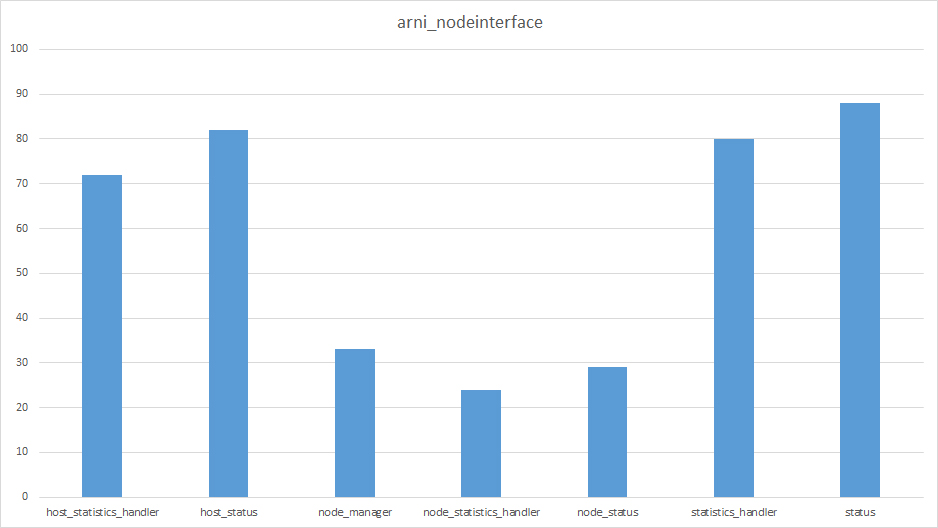
\includegraphics[scale=0.5]{./bilder/coverage/coverage_nodeinterface.jpg}
        \caption{Die dargestellten Daten wurden im Normalbetrieb des Nodeinterface Knotens erhoben, wobei �u�ere Zugriffe auf die Services nicht dargestellt werden konnten, weshalb entsprechende Bereiche unterrepr�sentiert sind.}
    \end{minipage}
    \hfill
\end{figure}  

\newpage
\section{Processing}

\begin{figure}[htbp]
    \begin{minipage}[t]{16cm}
        \vspace{0pt}
        \centering
        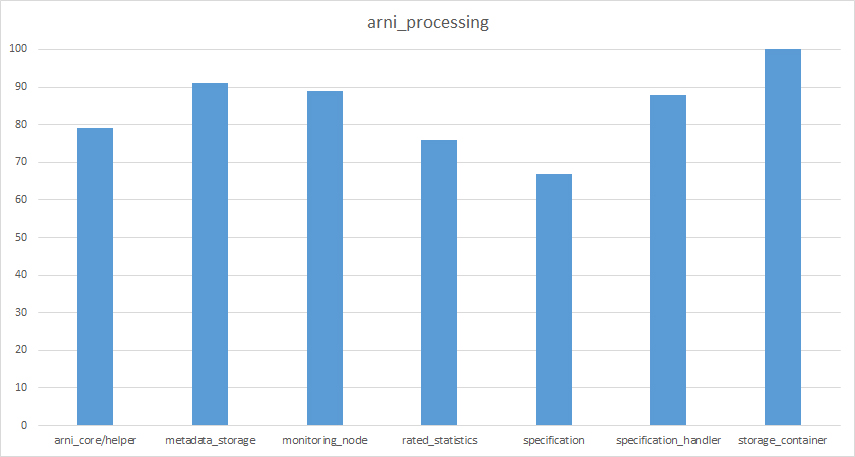
\includegraphics[scale=0.5]{./bilder/coverage/coverage_processing.jpg}
        \caption{Zur Erhebung der dargestellten Daten liefen mehrere Knoten (arni\_core/tutorial\_*) und ein Nodeinterface. Nachtr�glich wurde die GUI gestartet, die sich Daten �ber einen Service holte. Au�erdem wurden verz�gert Spezifikationen geladen, die auch einen Service bnuzten. Nach einer Weile wurde ein Knoten abgeschaltet, woraufhin Nachrichten �ber seine Fehlfunktion gesendet wurden.}
    \end{minipage}
    \hfill
\end{figure}  

\newpage
\section{Countermeasure}

\begin{figure}[htbp]
    \begin{minipage}[t]{16cm}
        \vspace{0pt}
        \centering
        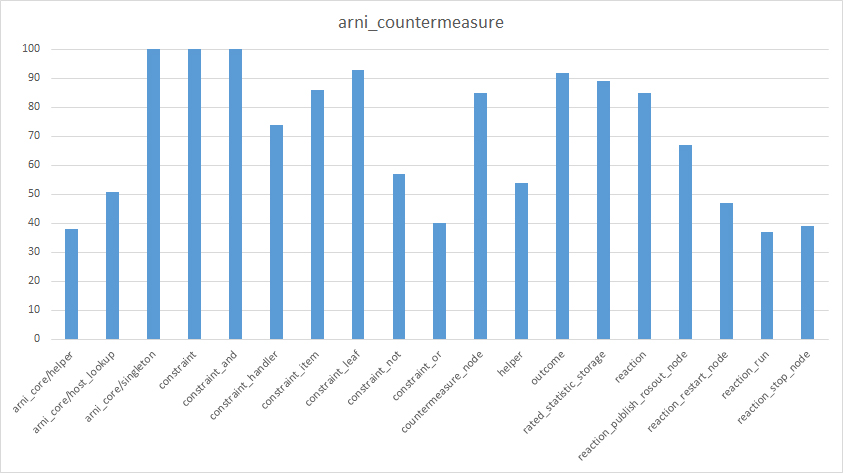
\includegraphics[scale=0.55]{./bilder/coverage/coverage_countermeasure4.jpg}
        \caption{Die dargestellten Werte wurden erreicht, indem Integrationstest 4 durchgef�hrt wurde.}
    \end{minipage}
    \hfill
\end{figure}  